%!TEX root = ../report.tex
\section{System context}
The system context is a fundamental artifact in the software architecture of a system. Developing the system context view is important, because this view is used as a mechanism to trace back to the business context, and downstream to the functional and operational architecture.

\subsection{Diagram}
The system context diagram of the system is outlined in \autoref{fig:system-context-diagram}.

\begin{figure}[H]
\centering
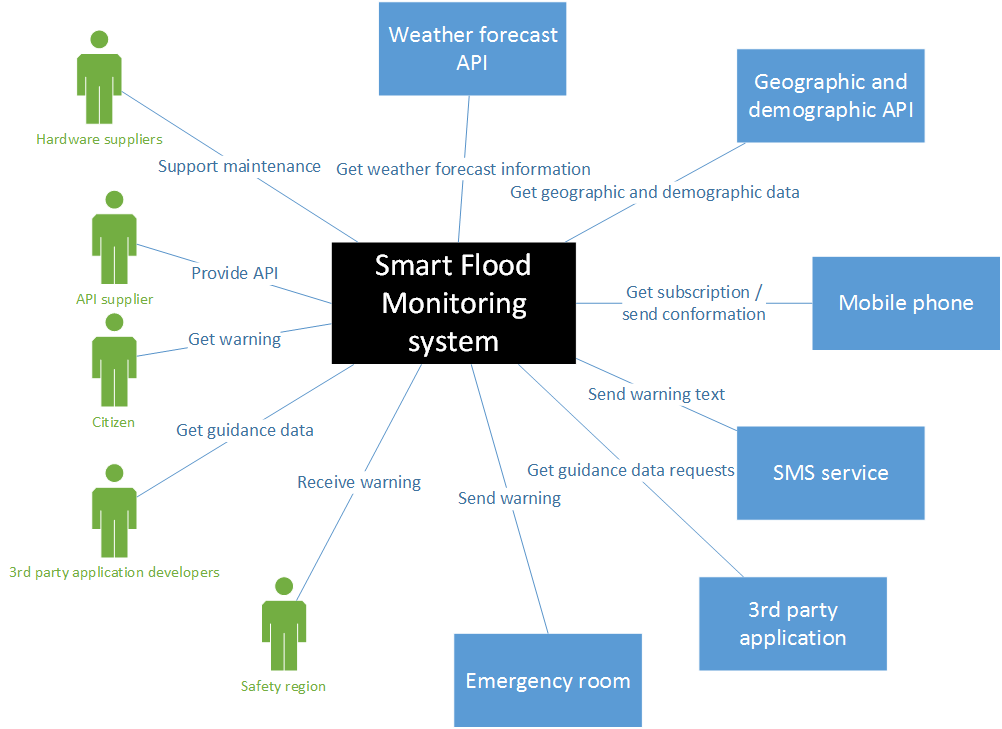
\includegraphics[keepaspectratio=true,width=0.7\textwidth]{images/system_context.png}
\caption{System context diagram}
\label{fig:system-context-diagram}
\end{figure}

\subsection{Users and Roles}
\begin{description}
	\item[Safety region] 
	\item[Citizens] In this system, citizens can be categorized into two group. First, citizens who do not subscribe to the service offered by the system. Second, citizens who subscribe the service. Indeed, Government will notify every citizens in affected areas. However, with subscription citizens can obtain more information regarding the flood and how to be safe.
	\item[Third party application developers] This user will also play an important role in case of floods. Emergency services will also be notified in case of imminent flood --- the government will notify them. Emergency services will also save the people and will be present in the affected areas.
	\item[Hardware suppliers] This user will also play an important role in case of floods. Emergency services will also be notified in case of imminent flood --- the government will notify them. Emergency services will also save the people and will be present in the affected areas.
\end{description} 

\subsection{External Systems}
\begin{description}
	\item[Weather Forecast API] The system will utilize weather forecast services from third party sources. To make this input reliable, the system uses multiple weather forecast providers. To predict floods correctly the system will need: rain data, temperature data, tides data, airpressure data and wind data.
	\item[Geographic and demographic API] To predict how floods will evolve over time, we need geographical data. This data consists of maps of the area. There are multiple parameters that are needed by the system: ground height, roads and waterways. To calculate the impact of an imminennt flood on society, we also need to know how many people live in the affected area. This data is retrieved through the demographic API.
	\item[Mobile phone] The mobile phone is a communication device of the citizen. This means a citizen uses the mobile phone to subscribe to the SMS service and to receive warnings in case of an imminent flood. This means the mobile phone should be able to send and receive text messages.
	\item[SMS service] The SMS system will communicate with the system and the mobile phones of the citizens. The SMS service keeps a list with all phone numbers that are subscribed to the service. When a warning is triggered by the central system, the SMS service gets a notification about this and sends the appropriate warning to the mobile phones that are within the area that is affected by the imminent flood.
	\item[Third party application] To guide citizens to a safe area in case of an imminent flood, we rely on third party applications. These applications get data from our API and deliver an app for citizens that provides guidance to a safe area.
	\item[Emergency room API] In case of an imminent flood we need to warn the safety region. This is done by invoking the emergency room API. In this way we send a message to the emergency room, which in their turn distributes this warning to the safety region.
\end{description}

\subsection{Channels and Information Flows}
\begin{table}[!htbp]
	\centering
    \begin{tabular}{L{\tw{0.2}} L{\tw{0.4}}}
    \toprule
    \multicolumn{2}{c}{$SFM\: \Leftrightarrow \: Weather \: forecast \: API$} \\ \midrule
    \textbf{Description} & The \ProjectName{} gets temperature, water pressure, and shifting information from sensors in dykes. \\
    \textbf{Connection} & Wireless, Internet \\
    \textbf{Protocol} & 4G \\
    \textbf{Data Volume} & Real time \\
    \bottomrule
    \end{tabular}
\end{table}

\begin{table}[!htbp]
	\centering
    \begin{tabular}{L{\tw{0.2}} L{\tw{0.4}}}
    \toprule
    \multicolumn{2}{c}{$SFM \: \Leftrightarrow \: Geographic \: and \: demographic \: API$} \\ \midrule
    \textbf{Description} & The \ProjectName{} gets temperature, water pressure, and shifting information from sensors in dykes. \\
    \textbf{Connection} & Wireless, Internet \\
    \textbf{Protocol} & 4G \\
    \textbf{Data Volume} & Real time \\
    \bottomrule
    \end{tabular}
\end{table}

\begin{table}[!htbp]
	\centering
    \begin{tabular}{L{\tw{0.2}} L{\tw{0.4}}}
    \toprule
    \multicolumn{2}{c}{$SFM \: \Leftrightarrow \: Mobile \: Phone$} \\ \midrule
    \textbf{Description} & The \ProjectName{} gets temperature, water pressure, and shifting information from sensors in dykes. \\
    \textbf{Connection} & Wireless, Internet \\
    \textbf{Protocol} & 4G \\
    \textbf{Data Volume} & Real time \\
    \bottomrule
    \end{tabular}
\end{table}
\begin{table}[!htbp]
	\centering
    \begin{tabular}{L{\tw{0.2}} L{\tw{0.4}}}
    \toprule
    \multicolumn{2}{c}{$SFM \: \Leftrightarrow \: SMS \: Service$} \\ \midrule
    \textbf{Description} & The \ProjectName{} gets temperature, water pressure, and shifting information from sensors in dykes. \\
    \textbf{Connection} & Wireless, Internet \\
    \textbf{Protocol} & 4G \\
    \textbf{Data Volume} & Real time \\
    \bottomrule
    \end{tabular}
\end{table}
\begin{table}[!htbp]
	\centering
    \begin{tabular}{L{\tw{0.2}} L{\tw{0.4}}}
    \toprule
    \multicolumn{2}{c}{$SFM \: \Leftrightarrow \: Third \: party \: application$} \\ \midrule
    \textbf{Description} & The \ProjectName{} gets temperature, water pressure, and shifting information from sensors in dykes. \\
    \textbf{Connection} & Wireless, Internet \\
    \textbf{Protocol} & 4G \\
    \textbf{Data Volume} & Real time \\
    \bottomrule
    \end{tabular}
\end{table}
\begin{table}[!htbp]
	\centering
    \begin{tabular}{L{\tw{0.2}} L{\tw{0.4}}}
    \toprule
    \multicolumn{2}{c}{$SFM \: \Leftrightarrow \: Emergency \: room \: API$} \\ \midrule
    \textbf{Description} & The \ProjectName{} gets temperature, water pressure, and shifting information from sensors in dykes. \\
    \textbf{Connection} & Wireless, Internet \\
    \textbf{Protocol} & 4G \\
    \textbf{Data Volume} & Real time \\
    \bottomrule
    \end{tabular}
\end{table}


\subsection{Alternatives}

\subsubsection*{Wired Connections}
Sensors will send real time information about the dykes and waterways to the Sensor monitoring block. The system will mostly use wireless connection to push the information gathered by sensors. Wired connection can also be used to send the information. However, this option needs physical connection between sensor monitoring and the sensors itself which will make the production cost way bigger since there will be many sensors installed. Thus, the wireless connection is the most feasible method.
